%%%%%%%%%%%%%%%%%%%%%%%%%%%%%%%%%%%%%%%%%
% Beamer Presentation
% LaTeX Template
% Version 1.0 (10/11/12)
%
% This template has been downloaded from:
% http://www.LaTeXTemplates.com
%
% License:
% CC BY-NC-SA 3.0 (http://creativecommons.org/licenses/by-nc-sa/3.0/)
%
%%%%%%%%%%%%%%%%%%%%%%%%%%%%%%%%%%%%%%%%%

%----------------------------------------------------------------------------------------
%	PACKAGES AND THEMES
%----------------------------------------------------------------------------------------

\documentclass[aspectratio=169,usenames,dvipsnames]{beamer}

\usepackage[utf8]{inputenc}
\usepackage{booktabs}
\usepackage{tabularx}
\usepackage[authordate,bibencoding=auto,strict,backend=biber,natbib]{biblatex-chicago}
\addbibresource{bib.bib}
\usepackage{graphicx}
% \hypersetup{
%     colorlinks,
%     %citecolor=black,
%     linkcolor=black
% }
\usepackage{array}
\usepackage{caption}
\usepackage{threeparttable}
\usepackage{epigraph} 
\usepackage{lscape}
\usepackage{adjustbox}
\newcommand*{\Scale}[2][4]{\scalebox{#1}{\ensuremath{#2}}}%
\usepackage{import}
\newenvironment{wideitemize}{\itemize\addtolength{\itemsep}{10pt}}{\enditemize}
\usepackage{amsmath}
\usepackage{csvsimple}
\usepackage{siunitx}
\usepackage{filecontents}
\usepackage{rotating}
\usepackage{multirow}
\usepackage{amsmath}
\usepackage{subcaption}
\usepackage{appendixnumberbeamer}
\usepackage{float}
\usepackage{amsmath}
\usepackage{csvsimple}
\usepackage{hyperref}
\newtheorem{proposition}{Proposition}
\usepackage{xcolor}
\def\boxit#1#2{%
    \smash{\color{red}\fboxrule=1pt\relax\fboxsep=2pt\relax%
    \llap{\rlap{\fbox{\phantom{\rule{#1}{#2}}}}~}}\ignorespaces
}
\newenvironment{variableblock}[3]{%
  \setbeamercolor{block body}{#2}
  \setbeamercolor{block title}{#3}
  \begin{block}{#1}}{\end{block}}
\usepackage{appendixnumberbeamer}
\usepackage{tikz,pgfplots}
\usepackage{tkz-fct}
\usepackage{amsthm}
\pgfplotsset{compat=1.10}
\usepgfplotslibrary{fillbetween}
\mode<presentation> {
\AtBeginSection[]
{
    \begin{frame}
        \frametitle{Table of Contents}
        \tableofcontents[currentsection]
    \end{frame}
}
% The Beamer class comes with a number of default slide themes
% which change the colors and layouts of slides. Below this is a list
% of all the themes, uncomment each in turn to see what they look like.

\usetheme{default}
%\usetheme{AnnArbor}
%\usetheme{Antibes} -
%\usetheme{Bergen}
%\usetheme{Berkeley}
%\usetheme{Berlin}
%\usetheme{Boadilla}
%\usetheme{CambridgeUS}
%\usetheme{Copenhagen} -
%\usetheme{Darmstadt}
%\usetheme{Dresden}
%\usetheme{Frankfurt}
%\usetheme{Goettingen}
%\usetheme{Hannover}
%\usetheme{Ilmenau}
%\usetheme{JuanLesPins}
%\usetheme{Luebeck}
%\usetheme{Madrid}
%\usetheme{Malmoe}
%\usetheme{Marburg}
%\usetheme{Montpellier}
%\usetheme{PaloAlto}
%\usetheme{Pittsburgh}
%\usetheme{Rochester} -
%\usetheme{Singapore}
%\usetheme{Szeged}
%\usetheme{Warsaw}

% As well as themes, the Beamer class has a number of color themes
% for any slide theme. Uncomment each of these in turn to see how it
% changes the colors of your current slide theme.

%\usecolortheme{albatross}
%\usecolortheme{beaver}
%\usecolortheme{beetle}
%\usecolortheme{crane}
%\usecolortheme{dolphin}
%\usecolortheme{dove}
%\usecolortheme{fly}
%\usecolortheme{lily}
%\usecolortheme{orchid}
%\usecolortheme{rose}
%\usecolortheme{seagull}
%\usecolortheme{seahorse}
%\usecolortheme{whale}
%\usecolortheme{wolverine}

%\setbeamertemplate{footline} % To remove the footer line in all slides uncomment this line
%\setbeamertemplate{footline}[frame number] % To replace the footer line in all slides with a simple slide count uncomment this line
\setbeamertemplate{theorems}[numbered]
\setbeamertemplate{navigation symbols}{} % To remove the navigation symbols from the bottom of all slides uncomment this line
}
\setbeamertemplate{caption}{\raggedright\insertcaption\par}
  \setbeamertemplate{enumerate items}[default]
  %\setbeamertemplate{page number in head/foot}{\insertframenumber}
\usepackage{graphicx} % Allows including images
\usepackage{booktabs} % Allows the use of \toprule, \midrule and \bottomrule in tables
%\usepackage {tikz}
\newtheorem*{theorem*}{Theorem}
\newtheorem*{lemma*}{Lemma}
\newtheorem*{proposition*}{Proposition}
\newtheorem*{corollary*}{Corollary}
\newtheorem*{definition*}{Definition}
\DeclareMathOperator*{\argmin}{arg\,min}
\newtheorem*{assumption}{Assumption}
\usetikzlibrary {positioning}
\renewcommand{\arraystretch}{1.5}
\newcommand\hideit[1]{%
  \only<0| handout:1>{\mbox{}}%
  \invisible<0| handout:1>{#1}}
\usepackage[default]{lato}

\setbeamercolor{block body alerted}{bg=alerted text.fg!10}
\setbeamercolor{block title alerted}{bg=alerted text.fg!20}
\setbeamercolor{block body}{bg=structure!10}
\setbeamercolor{block title}{bg=structure!20}
\setbeamercolor{block body example}{bg=green!10}
\setbeamercolor{block title example}{bg=green!20}


\makeatletter
\let\save@measuring@true\measuring@true
\def\measuring@true{%
  \save@measuring@true
  \def\beamer@sortzero##1{\beamer@ifnextcharospec{\beamer@sortzeroread{##1}}{}}%
  \def\beamer@sortzeroread##1<##2>{}%
  \def\beamer@finalnospec{}%
}
\makeatother
%\usepackage {xcolor}

%----------------------------------------------------------------------------------------
%	TITLE PAGE
%----------------------------------------------------------------------------------------

\title[diss]{Lecture 6: Does Performance Pay Work?} % The short title appears at the bottom of every slide, the full title is only on the title page
\author{Compensation in Organizations} % Your name
\institute[shortinst]{Jacob Kohlhepp}
\date{\today} % Date, can be changed to a custom date

\begin{document}

\begin{frame}
\titlepage % Print the title page as the first slide

\end{frame}


\begin{frame}{Thinking Through the Theory}
\begin{wideitemize}
    \item We found that performance-pay works less well compared to effort-based pay.
    \item But effort-based pay is usually infeasible!
    \item So if we want to know if performance-pay works we should not compare the two.
    \item Instead we should ask: does forcing the firm to not use performance pay reduce surplus?
\end{wideitemize}
    
\end{frame}

\begin{frame}{Thinking Through the Theory}
\begin{wideitemize}
    \item Question: What does no performance pay mean?

    \pause
    \begin{wideitemize}
        \item Answer: $\beta=0$
    \end{wideitemize}
    \pause
    \item How does this impact worker effort?
\end{wideitemize}
    
\end{frame}

\begin{frame}{Thinking Through the Theory}
\begin{wideitemize}
    \item If $\beta=0$ then the benefit to the worker of effort is $0$.
    \item But the marginal cost is positive!
    \item Therefore exert no effort $e=0$
    \item In math: For $e>0$, we have $c'(e)>0=\beta \implies e=0$.
\end{wideitemize}


\end{frame}
\begin{frame}{Thinking Through the Theory}
\begin{wideitemize}
    \item So effort is $0$.
    \item What is profit from $\beta=0$ (no performance pay)?\pause 
  \begin{align*}
        \pi_{\beta=0} &= E[y-w(y)]\\
        &=e - \alpha - \beta e\\
        &= 0 - \alpha - 0\cdot 0\\
        &=-\alpha
    \end{align*}
    \pause
    \item But we still need the worker to take the job.
    \item Therefore we need $\alpha\geq \bar u$
    \item Therefore the best we can do is $\alpha=\bar u$
    \item Therefore profit is $-\bar u$    
    
\end{wideitemize}


\end{frame}
\begin{frame}{Thinking Through the Theory}
\begin{wideitemize}
    \item So $\pi_{\beta=0}=-\bar u$
    \item Assume $\bar u>0$, we are better off setting $\alpha = -\infty$
    \item Then the worker does not take the job and the firm makes $0>\pi_{\beta=0}=-\bar u$
    \item Performance pay has positive profit, so: $\pi_p>-\bar u=\pi_{\beta=0}$
    \begin{wideitemize}
    \item To see this clearly just plug in $c(e)=e^2/2$
    \item Then $\pi_p=\frac{1}{2}\frac{1}{1+r\sigma^2}-\bar u$.
    \item This is more than $-\bar u$
    \end{wideitemize}
\end{wideitemize}


\end{frame}



\begin{frame}{Thinking Through the Theory}

\begin{wideitemize}
    \item The theory unambiguously says that performance pay is better than no performance pay.
     \item Another way to see this is it just remember this theorem:
    \begin{theorem*}
        When wages depend only on output, effort is $e_{p}$ which solves 
        \[c'(e_{p})= \frac{1}{1+r \sigma^2 c''(e_{p})}\]
        and $\beta_{p} =c'(e_{p}),\alpha_{p} =\bar u - \beta_{p} e_{p}+r \beta^2\sigma^2/2+c(e_{p})$.
    \end{theorem*}
\item  We showed that the firm maximizes total surplus.
\item The firm could have chosen $\beta=0$ but it doesn't, so total surplus must be larger with performance pay than without it!
\end{wideitemize}
\end{frame}

\section{Empirical Evidence}


\begin{frame}
\centering
    \huge Discussion: Muralidharan and Sundararaman (2011)
\end{frame}

\begin{frame}{``Teacher Performance Pay: Experimental Evidence from India"}
    \begin{wideitemize}
        \item This is Muralidharan and Sundararaman (2011).
        \item Motivation: Research shows rewarding based on teacher characteristics like tenure and master's degrees does not improve outcomes.
        \item Concern: other work highlights the possibility of perverse outcomes.
        \begin{wideitemize}
            \item Neal and Schanzenbach (2010): teachers focused attention on students in the middle of the distribution
            \item Question: how does this compare to another paper we read?
        \end{wideitemize}
        \item Research method: randomized control trial in India.
        \item Group bonuses vs. individual bonuses vs. nothing
        \item Bonuses are on average 3 annual salary.
    \end{wideitemize}
\end{frame}

\begin{frame}{``Teacher Performance Pay: Experimental Evidence from India"}
    \begin{wideitemize}
        \item 300 schools, with 100 in each treatment group.
        \item 0.27 (math) and 0.17 (lang.) std. dev. improvements vs. control group
        \item Gains are ``broad-based" across academic achievement distirbution (what does this mean?)
        \item Also gains in social studies and science (why is this interesting?)
        \item Individual incentives worked better in the long term than group, but were the same in the short term (why might this be?)
    \end{wideitemize}
\end{frame}

\begin{frame}{``Teacher Performance Pay: Experimental Evidence from India"}
    \begin{wideitemize}
        \item 100 additional schools were given more money to get more supplies
        \item 100 additional, additional schools were given more money to hire extra teachers.
        \item These 200 schools had better test scores (+0.08 st. dev.).
        \item But performance pay improved scores more for less money.
    \end{wideitemize}
\end{frame}




\begin{frame}{``Teacher Performance Pay: Experimental Evidence from India"}
Why is sample balance important?

    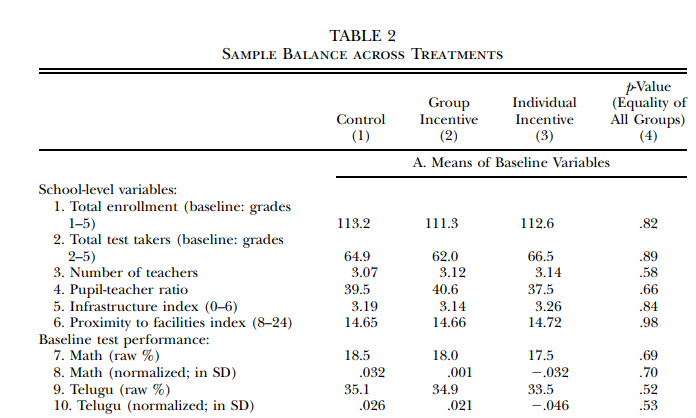
\includegraphics[width=0.7\textwidth]{pictures/balance_teachers.png}
\end{frame}

\begin{frame}{``Teacher Performance Pay: Experimental Evidence from India"}
Why would attrition be concerning?

    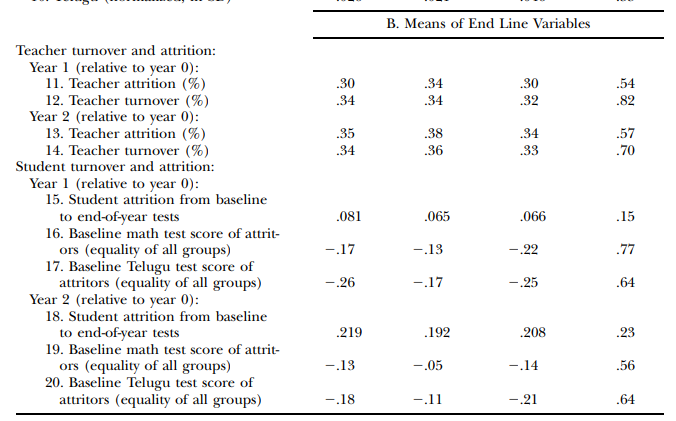
\includegraphics[width=0.7\textwidth]{pictures/balance_teachers_end.png}
\end{frame}

\begin{frame}{``Teacher Performance Pay: Experimental Evidence from India"}
Why is sample balance important?

    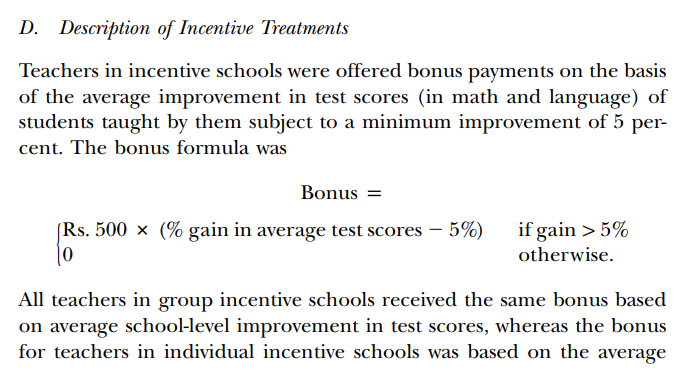
\includegraphics[width=0.7\textwidth]{pictures/bonus_scheme_teachers.png}
\end{frame}

\begin{frame}{``Teacher Performance Pay: Experimental Evidence from India"}
Why is sample balance important?

    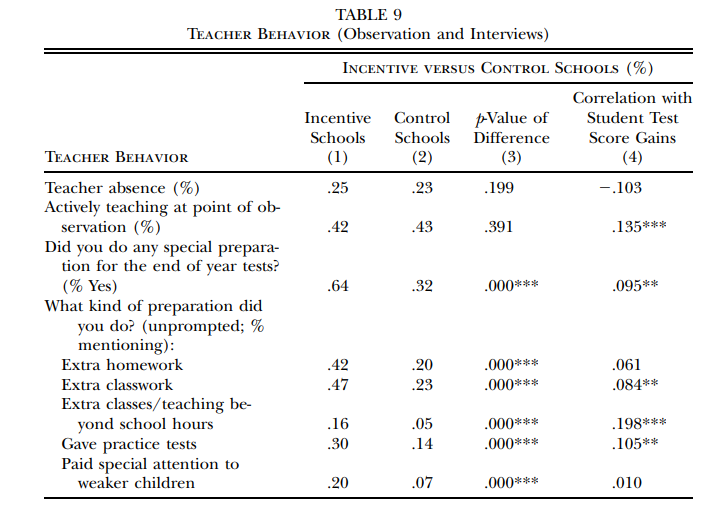
\includegraphics[width=0.7\textwidth]{pictures/teacher_behavior.png}
\end{frame}




\begin{frame}{``Teacher Performance Pay: Experimental Evidence from India"}
    \begin{wideitemize}
        \item This paper has many nice features\pause
        \item Turnover and transfer of teachers are shown to have no discernible impact.
        \item Exams were given by external teams, tudent identities were verified.
        \item Results are shown by type of question (multiple choice, repeat)
        \item Teacher behavior was measured ($\beta \uparrow \implies e\uparrow \implies y \uparrow$)
    \end{wideitemize}
\end{frame}


\begin{frame}{``Performance Pay and Productivity"}
    \begin{wideitemize}
        \item This is Lazear (2000)
        \item Safelite Glass Corporation installs automobile glass
        \item In 1994, they switched from hourly pay to a piece rate system
        \item This is performance pay: worker wage depends on output
        \item Data: 3,000 workers and 19 month period
        \item Productivity Measure: units-per-worker-per-day
    \end{wideitemize}
\end{frame}



\begin{frame}{``Performance Pay and Productivity"}
\centering
    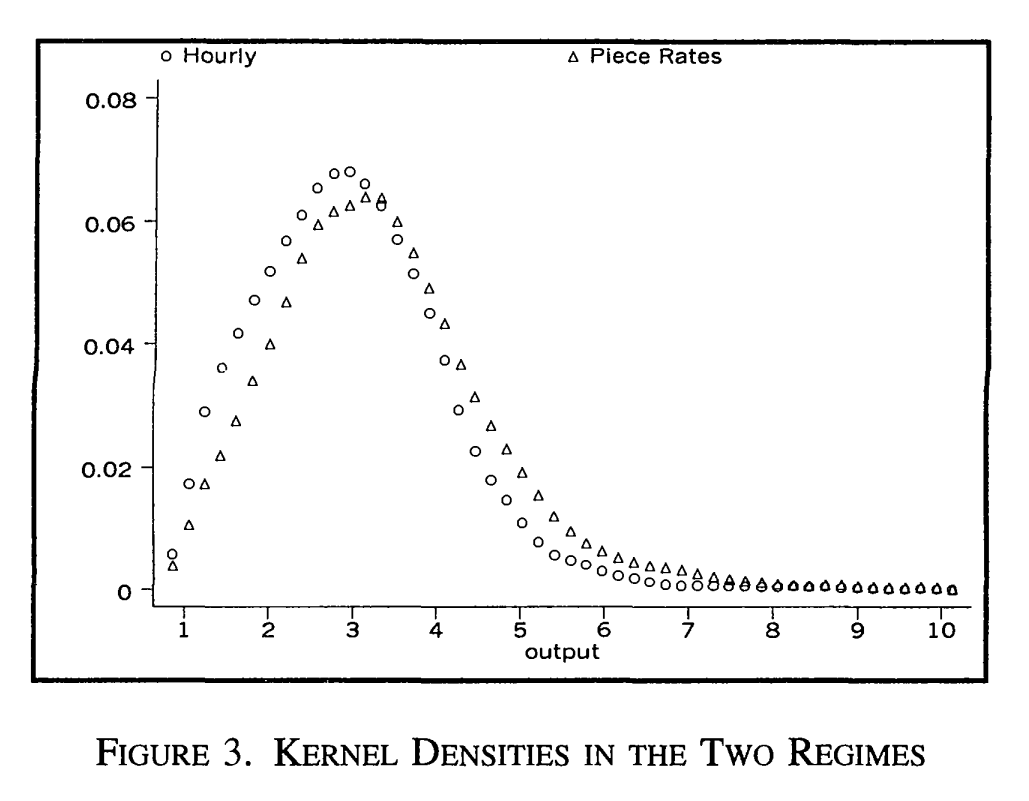
\includegraphics[width=0.7\textwidth]{pictures/safelite.png}
\end{frame}


\begin{frame}{``Performance Pay and Productivity"}
\centering
    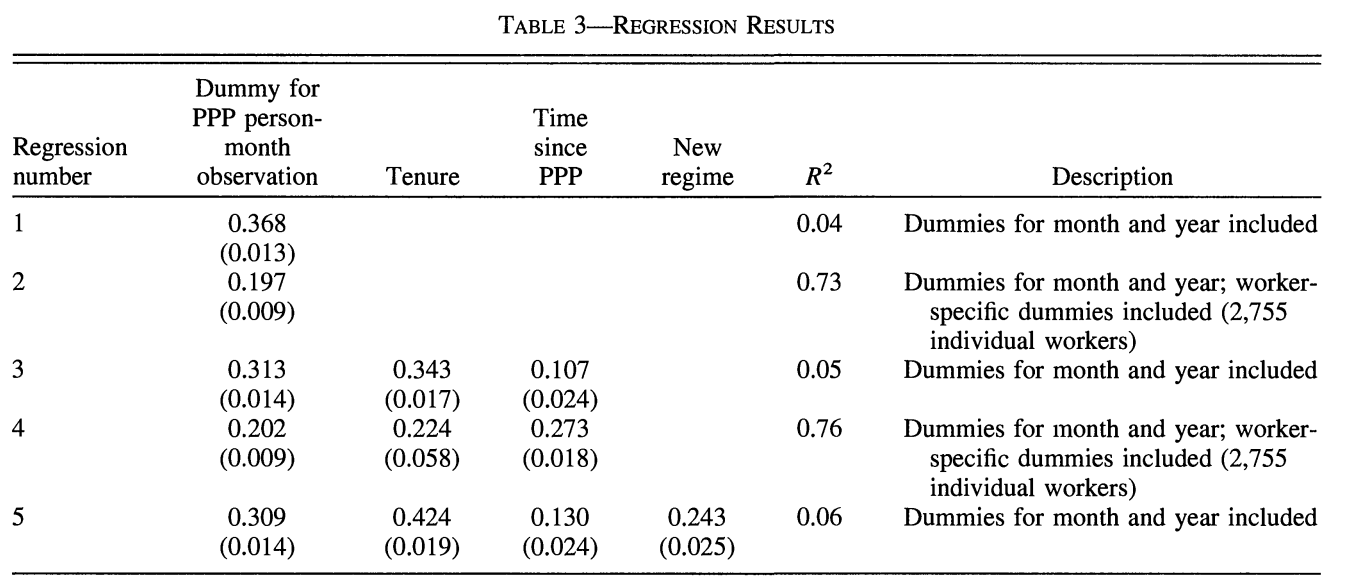
\includegraphics[width=0.7\textwidth]{pictures/safelite_table.png}
    
    Productivity increased by 44 percent (first coef. divided by the pre-performance pay mean)
\end{frame}


\begin{frame}{``Performance Pay and Productivity"}
    \begin{wideitemize}
        \item Workers hired under pay for performance system are more productive.
        \item Pay increased by 7 percent.
        \item Profit likely rose: 44\% productivity increase vs. 7 percent pay increase.
    \end{wideitemize}
\end{frame}




\begin{frame}{``It’s Not What You Pay it’s the Way that You Pay it and that’s What Gets Results: Jockeys’ Pay and Performance" }
    \begin{wideitemize}
        \item This is Fernie and Metcalf (1999).
        \item Setting: horseracing jockeys
        \item Three big findings:

        \begin{wideitemize}
            \item Incentives and monitoring mechanisms are used to align jockey's interests with their firm.
            \item Pay and performance are positively associated.
            \item Performance is better under performance pay than flat fees.
        \end{wideitemize}
    \end{wideitemize}
\end{frame}


\begin{frame}{Fernie and Metcalf (1999): Setting }
    \begin{wideitemize}
        \item 109 full jockeys, 201 apprentices.
        \item Supply of jockeys is purposefully restricted, jockeys cannot be replaced by capital.
        \item Demand for horseracing was stable throughout the period.
        \item Jockey pay was between 2-3 of total costs of horse owners.
        \item Effort is hard to measure: jockey can attribute bad performance to the horse
        \item Jockeys can be bribed by a bookie.        
    \end{wideitemize}
\end{frame}

\begin{frame}{Fernie and Metcalf (1999): Measuring Performance }
    \begin{wideitemize}
        \item    One option: return to placing a dollar bet on all horses the jockey rode in a season.
        \item Problem: returns are driven by many other factors and are well udnerstood not to reflect the jockey's performance.
        \item Other option: total wins
        \item Problem: Big confounding factor is the horse and the matching between horses and riders
        \item Fix: system of separating horse effect and rider effect.
    \end{wideitemize}
\end{frame}





\begin{frame}{Fernie and Metcalf (1999): Non-Performance Pay }
    \begin{wideitemize}
        \item    For some jockeys, there was a switch to non-performance pay.
        \item `Mega-rich owners" retained certain jockeys by paying sums of up to 1 million pounds.
        \item The payments did not depend on performance.
        \item We can compare performance before and after switch to non-performance pay.
        \item This accounts for the selection margin (why is this an issue?)
        \item They find worse performance, in line with out theory ($\beta=0 \implies e=0$)
    \end{wideitemize}
\end{frame}




\begin{frame}{More Evidence that Performance Pay Boosts Productivity}
\begin{wideitemize}
    \item We looked at windshield installers, teachers, ministers, jockeys, doctors.
    \pause
    \item But other papers show evidence in other settings:
        \begin{wideitemize}
        \item Paarsch and Shearer (1996): Canadian tree planters
        \item Banker, Lee, and Potter (1996): retail sales
        \item Andrew Foster and Mark Rosenzweig (1994): farmers in the Phillipines
        \item  Larry Kahn and Peter Sherer (1990): white-collar office workers
        \item Question: What do these jobs have in common?
    \end{wideitemize}
\end{wideitemize}

\end{frame}


\begin{frame}{Summarizing Empirical Evidence}
\begin{wideitemize}
    \item Performance pay improves performance ($\beta\uparrow \implies e \uparrow$)
    \item But other implications are mixed.
    \item In particular the risk incentive trade-off ($\sigma^2 \uparrow \not \implies \beta \downarrow$)
\end{wideitemize}

\pause
\begin{block}{``The Provision of Incentives in Firms" (Prendergast 1999) }
    ``This paper provides an overview of the existing theoretical and empirical work on the provision of incentives. It reviews the costs and benefits of many types of pay-for-performance, such as piece rates, promotions, and long-term incentives. The main conclusions are (i) while there is considerable evidence that individuals respond to pay-for-performance, there is less evidence that contracts are designed as predicted by the theory, (ii) there has been little progress made in distinguishing amongst plausible theories, and (iii) we still know little about how incentives are provided to workers whose output is difficult to measure."
\end{block}
    
\end{frame}



\end{document}







